\begin{figure}
\centering
\begin{subfigure}[b]{0.75\linewidth}
    \hfill
    \includegraphics[height=7em]{explainer/adm_10_size}
    \caption{~The second dataset without diagnoses ordered by ``total" size.}
    \label{figs:adm_10_size}
\end{subfigure}
\\
\begin{subfigure}[b]{0.75\linewidth}
    \hfill
    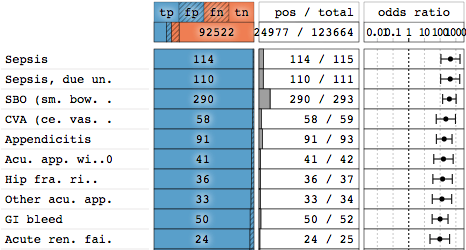
\includegraphics[height=7em]{explainer/adm_10_or_full}
    \caption{~The second dataset using diagnoses ordered by ``odds ratio".}
    \label{figs:adm_10_diag}
\end{subfigure}%
\caption{Showing the second dataset of the case study (Section~\ref{sec:case_study}) with and without using diagnoses features in the \textbf{\tabB}.}
\end{figure}
% \begin{figure}
% \centering
% \begin{subfigure}[b]{\linewidth}
%     \hfill
%     \includegraphics[height=9.5em]{fig/adm_10_size}
%     \caption{~The second dataset without diagnoses ordered by ``explanation length".}
%     \label{figs:adm_10_size}
% \end{subfigure}
% \\
% \begin{subfigure}[b]{1.01\linewidth}
%     \hfill
%     \includegraphics[height=9.5em]{fig/adm_10_diag}
%     \caption{~The second dataset (filtered by $total > 200$) using diagnoses ordered by ``odds ratio".}
%     \label{figs:adm_10_diag}
% \end{subfigure}%
% \\
% \begin{subfigure}[b]{\linewidth}
%     \hfill
%     \includegraphics[height=9.5em]{fig/adm_10_or_nodiag}
%     \caption{~The second dataset (filtered by $total > 200$) without diagnoses ordered by ``odds ratio".}
%     \label{figs:adm_10_or_nodiag}
% \end{subfigure}%
% \\
% \begin{subfigure}[b]{\linewidth}
%     \hfill
%     \includegraphics[height=9.5em]{fig/adm_10_or_ff}
%     \caption{~The first biased dataset (filtered by $total > 200$) ordered by ``odds ratio".}
%     \label{figs:adm_10_or_ff}
% \end{subfigure}
% \\
% \begin{subfigure}[b]{\linewidth}
%     \hfill
%     \includegraphics[height=16em]{fig/adm_ft}
%     \caption{~The second biased dataset ordered by ``incorrect".}
%     \label{figs:adm_ft}
% \end{subfigure}
% \caption{Datasets as they are discussed in Section~\ref{sec:case_study} and Section~\ref{sec:bias}.}
% \end{figure}